\chapter{Implementation} % Main chapter title

\label{Chapter3} % For referencing the chapter elsewhere, use \ref{Chapter3} 

In this chapter, the approaches used in this research is examined. First, the join dataset merging from Last.fm and Spotify is mentioned. After that, the three algorithms and the evaluation metrics are discussed in detail.

\section{Dataset}

\subsection{Dataset creation}
The dataset for this thesis is a combination between two databases from two services: the 1K users dataset from Last.fm \footnote{https://last.fm} and the dataset crawling from Spotify Web Api \footnote{https://developer.spotify.com/web-api}. 

The dataset from Last.fm contains the listening habit from February, 2005 until May, 2009 for nearly 1000 users. The dataset contains more than 19 million entries, each entry consists of 4 attributes: the user id from Last.fm, the song that the user listened to, the artist who wrote the song, and the timestamp represents the time the user listened to the song. 

From the last.fm dataset, top 10000 songs that have the highest listening frequency are choosen. Then, track name and the respective artist are queried on Spotify API to get the corresponding track features. As Spotify API not only returns exact match but also similar match, and the name convention between the two systems might be different, a fuzzy matching algorithm is applied to filter the results. Particularly, the Levenshtein ratio is applied on the two fields. Any matching with a ratio higher than 80 percent is a good match, since the two strings are basically the same with some minor differences, which are the results of the different convention between the two system. Since matches with ratio between 60 and 80 percent might be good ones, manual check was done to guarantee the best result. I decided to cut off the result at 60 percent, as the majority of matches that are less than 60 percent are noisy and not accurate.

As some of the songs from Last.fm have yet been analyzed by Spotify, after joining the two datasets, the number of remaining songs is about 4200. I then remove users with less than 10 listening events.
The dataset is then divided into training set and test set following this rule: for each user, split the listening time into two halves, of which the first half belongs to the training set and the second half belongs to the test set. In the test set, all the tracks that are listened only 1 time are eliminated, as it is likely that the user only listened to it by chance. The final dataset contains with 891 users, 4200 unique tracks, and ...

\noindent The final dataset contains the following fields:

\begin{itemize}
\item[•] Username: The user who listen to the album, taken from last.fm database.
\item[•] Album: The name of the album the user listens to.
\item[•] Artist: The artist who performs the album.
\item[•] Playcount: The total number of time the user listens to the album.
\item[•] TrackId: The unique id of the track in Last.fm dataset, which also serves as unique key.
\item[•] Energy: A perceptual measurement of intensity and activity in a range from 0 to 1. The higher the score, the higher the energy the track contains. For example, metal rock has high energy, while a Bach prelude is perceived to have low energy. This measurement is built on top of dynamic range, loudness, timbral, onset rate, and general entropy.
\item[•] Speechiness: A measurement of how much spoken words is present compare to music. A value from 0.66 to 1 indicates that the track is mostly spoken words, such as talk show or audio book. Vice versa, a value between 0.33 and 0.66 implies that the track contains both music and speech, ranging from pop to rap music. A value below 0.33 indicates a non speech track. 
\item[•] Acousticness: A evaluation of how much acoustic a track contains compare to how much electronic. Again, a value closer to 1 implements that the track is played with mostly acoustic instruments, such as guitar and harmonica; while a value closer to 0 implements the present of electronic instruments.
\item[•] Danceability: A measurement of how suitable a track is for dancing based on a combination of musical elements including tempo, rhythm stability,  beat strength, and overall regularity. The higher the value, the more danceable the track.
\item[•] Tempo: The overall estimated tempo of a track, measuring in beats per minute (BPM).
\item[•] Instrumentalness: The assessment of how much a track incorporates vocals. The higher the instrumentalness, the greater likelihood the track contains no vocal content. 
\item[•] Key: The key (tonal center) a track is in. Integers map to pitches using Pitch Class notation \footnote{https://en.wikipedia.org/wiki/Pitch\_class}. 
\item[•] Valence: A measure from 0 to 1 of the positiveness of a track. Tracks with high valence sound more positive (e.g. happy, cheerful), and vice versa.
\item[•] Liveness: An indication of whether a track is performed live or in studio. The higher the liveness, the higher possibility that the track is performed live.
\item[•] Loudness: The overall loudness of a track in decibels (dB), with range from -60 to 0 db. 
\item[•] Mode: An indication of modality (major or minor) of a track. The field has only 2 values: 1 for major and 0 for minor.
\item[•] Time signature: An indication of how many beats are in each bar of a track. 
\end{itemize}

\subsection{Some descriptive data summarization}

In this section, some basic descriptive statistics of the data will be described, in order for the understanding of the overall picture of the data. Figure \ref{fig:boxplot} represent the boxplot diagrams of the energy, speechiness, acousticness, danceability, tempo, instrumentalness, valence, liveness, and loudness respectively. For key, mode, and time signature, as they are categorical variables, boxplot diagram information is not useful. Instead, for these variables, the frequency of the values, such as in table \ref{fig:freq_table} is displayed.

\begin{figure}
  \begin{subfigure}[b]{0.3\textwidth}
    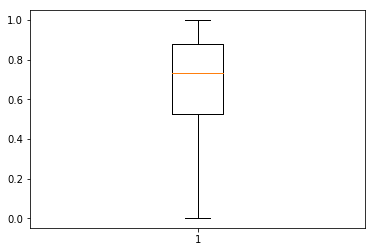
\includegraphics[width=\textwidth]{energy}
    \caption{Energy}
    \label{fig:energy}
  \end{subfigure}
  \hfill
  \begin{subfigure}[b]{0.3\textwidth}
    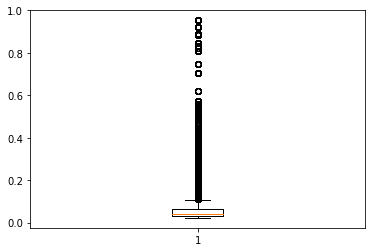
\includegraphics[width=\textwidth]{speechiness}
    \caption{Speechiness}
    \label{fig:speechiness}
  \end{subfigure}
  \hfill
  \begin{subfigure}[b]{0.3\textwidth}
    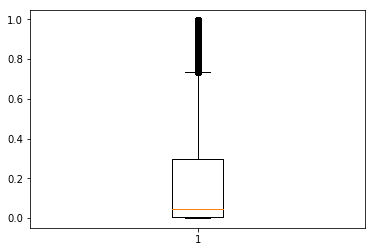
\includegraphics[width=\textwidth]{acousticness}
    \caption{Acousticness}
    \label{fig:acousticness}
  \end{subfigure}
  
  \bigskip
    \begin{subfigure}[b]{0.3\textwidth}
    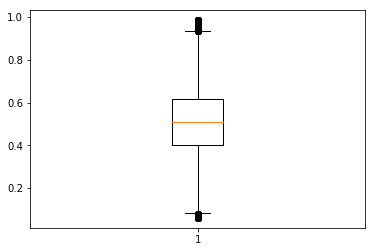
\includegraphics[width=\textwidth]{danceability}
    \caption{Danceability}
    \label{fig:danceability}
  \end{subfigure}
  \hfill
    \begin{subfigure}[b]{0.3\textwidth}
    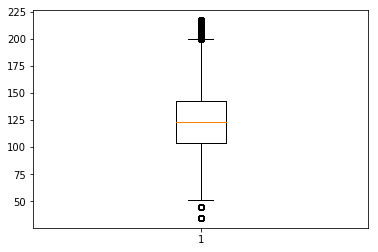
\includegraphics[width=\textwidth]{tempo}
    \caption{Tempo}
    \label{fig:tempo}
  \end{subfigure}
  \hfill
    \begin{subfigure}[b]{0.3\textwidth}
    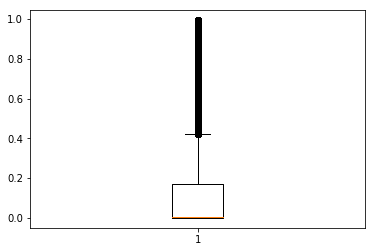
\includegraphics[width=\textwidth]{instrumentalness}
    \caption{Instrumentalness}
    \label{fig:instrumentalness}
  \end{subfigure}
  
  \bigskip
      \begin{subfigure}[b]{0.3\textwidth}
    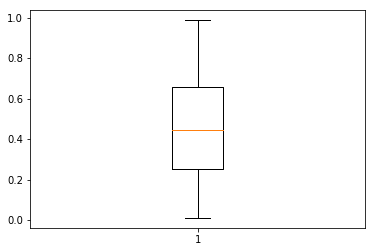
\includegraphics[width=\textwidth]{valence}
    \caption{Valence}
    \label{fig:valence}
  \end{subfigure}
  \hfill
    \begin{subfigure}[b]{0.3\textwidth}
    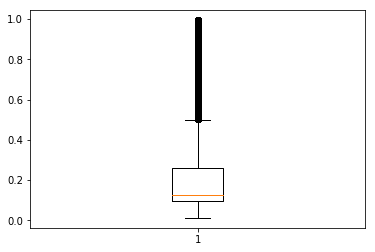
\includegraphics[width=\textwidth]{liveness}
    \caption{Liveness}
    \label{fig:liveness}
  \end{subfigure}
  \hfill
    \begin{subfigure}[b]{0.3\textwidth}
    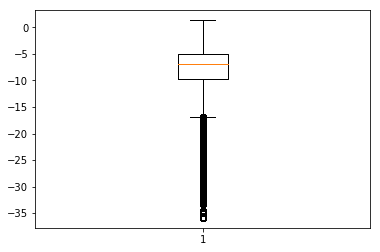
\includegraphics[width=\textwidth]{loudness}
    \caption{Loudness}
    \label{fig:loudness}
  \end{subfigure}
  
  \caption{Boxplot diagram of music features}
  \label{fig:boxplot}
\end{figure}

\begin{figure}
  \begin{subfigure}[b]{0.3\textwidth}
    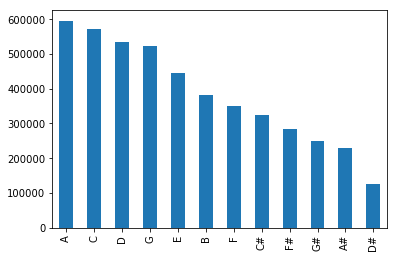
\includegraphics[width=\textwidth]{key}
    \caption{Key}
    \label{fig:key}
  \end{subfigure}
  \hfill
   \begin{subfigure}[b]{0.3\textwidth}
    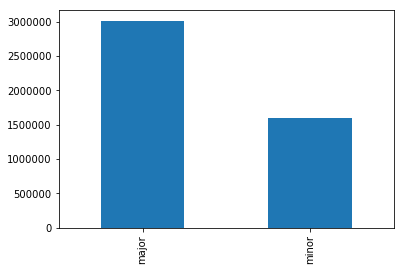
\includegraphics[width=\textwidth]{mode}
    \caption{Mode}
    \label{fig:mode}
  \end{subfigure}
  \hfill
  \begin{subfigure}[b]{0.3\textwidth}
    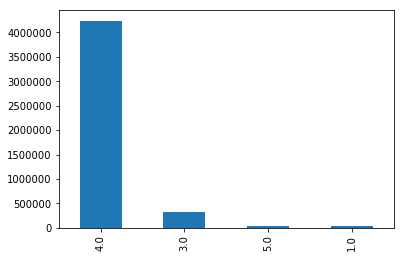
\includegraphics[width=\textwidth]{time_signature}
    \caption{Time signature}
    \label{fig:time_signature}
  \end{subfigure}
	
	\caption{Frequency table of music features}
	\label{fig:freq_table}
\end{figure}

\bigskip

\noindent We can see that from the diagrams:
\begin{itemize}
	\item Energy: the median is quite high, at nearly 0.8. However, the interquartile range of the energy is 0.35, suggesting that the energy spans equally across the value range.
	\item Speechiness: the median is at 0.04, with the first quartile at 0.03 and third quartile at 0.06, showing that most of the tracks have low level of spoken word. 
	\item Acousticness: the median is also at 0.04, with the first quartile at 0.003. However, the third quartile is at 0.3, suggesting that most of the tracks are not acoustic.
	\item Danceability: the median is at 0.5, with the first quartile at 0.4 and third quartile at 0.6, showing a normal distribution, which means that people listen equally to danceable track as well as undanceable track.
	\item Tempo: the median tempo is 123, with the first quartile of 104 and third quartile of 142, suggesting that most people listen to Allegro, which is fast and bright music.
	\item Instrumentalness: the median of 0.003 and the third quartile of 0.17 imply that most of the tracks contain vocal and not just pure instrument.
	\item Valence: with the median of 0.44, first quartile of 0.25, and third quartile of 0.66, valence also forms the normal distribution, suggesting that people listen equally to both positive and negative music.
	\item Liveness: the median of 0.12 and third quartile of 0.25 indicate that most tracks have a low level of liveness.
	\item Loudness: the first quartile of -9 and third quartile of -5 implement that most song have quite the same level of loudness.
	\item Key: songs with different key have different playing frequency. Overall, major key songs dominate minor ones.
	\item Mode: major key tracks are played more than minor ones, as previously stated.
	\item Time signature: the table indicates that more than 90\% of the tracks have 4 beats in each measure, around 7\% of the tracks have 3 beats in each measure, and the rest of the track have either 1 or 5 beats per measure.
\end{itemize}
	
\section{Algorithms}

The following sections describe my implementation of the three algorithms that are used in this thesis: a Na\"ive collaborative filtering, a collaborative filtering approach specified for implicit feedback dataset, followed by the hybrid approach that combine collaborative filtering with item features.

\subsection{Pure Collaborative Filtering}
As the number of song outnumbers the number of user, I decide to implement the user-user based collaborative filtering. The algorithm can be summarized in the following steps:

\begin{enumerate}
	\item Calculate similarity between users using cosine similarity between users' rating vectors. 
	\item For each user, form a neighborhood of \textit{n} users that have the highest similarity.
	\item Compute a prediction for an item from a weighted combination of selected neighbor's ratings. 
\end{enumerate}

In step 3, predictions are calculated using the weighted average of deviations from neighbors' mean. The formula is as follow:

\begin{displaymath}
p_{a,i} = \overline{r}_a + \frac{\sum_{u=1}^{n} (r_{u,i} - \overline{r}_{u}) \times P_{a,u}}{\sum_{u=1}^{n} P_{a,u}}  \tag{1} 
\end{displaymath}

with \(p_{a,i} \) is the prediction of item i for user a, \(P_{a,i}\) is the similarity between user a and user u, and \(\overline{r}_a\) is the average of the ratings of user a.  

\subsection{Collaborative Filtering for Implicit Feedback Dataset}

\subsubsection{Introduction}
One of the most well known work on implicit feedback dataset is the one of Yifan Hu et al \cite{hu2008collaborative}. In his paper, he mentioned that almost all the prior approaches were mostly designed for explicit feedback, and therefore applying these methods on implicit dataset might not work well. According to his work, there are four crucial differences between the two type of dataset:

\begin{enumerate}
	\item No negative feedback: In explicit feedback dataset, the users actively tell us which items they like and the ones that they do not. In implicit feedback, however, telling the items that the users dislike is hard to achieve. The reason is that, by observing the user behaviors, we can infer that the user might like the items that they consume. However, for an item that the user has no interaction with, it is unknown whether the user does not favor it or he does not know about its existence. This phenomenon derives a crucial implication: in explicit dataset, a pair of user - item that has no information is treated as missing data and is omitted from the analysis. This is impossible for implicit dataset, as eliminating these missing data would leave us with only positive feedback, greatly misrepresenting the full user profile. 
	
	\item Implicit feedback is noisy: passively tracking user behaviors can only give us indirect information about user preferences and true motives. For example, we may view purchase from a user, but this does not necessarily indicate a positive view of the product. The user might buy the item as a gift, or show disappointment only later the purchase. This leads to the third distinction.
	
	\item The numerical value of explicit feedback indicates preference, while the numerical value of implicit feedback indicates confidence: Explicit feedback let users express their level of preference, e.g. a scale between 1 (totally dislike the item) to 5 (totally love the item). In contrast, numerical values of implicit feedback describe the frequency of actions, e.g. how much time the user listens to a particular song or watches a show. A large value not necessarily implies that the user like the item. For example, in the film domain, a user might really like a movie but is hesitated to watch it again because of the lengthy duration. However, he might periodically watch a weekend show, which derives from his habit but not appreciation of the show. 
	
	\item Evaluation of implicit-feedback recommender requires appropriate measures. Traditionally, metrics such as mean squared error are often applied to measure the success of the recommender. However, in implicit models we have to also consider the available of the items, or the competition between items. For example, it is unclear how to evaluate two shows that are on at the same time, and hence cannot be both watched by the user.
\end{enumerate}

The above comments are used to make adjustments to traditional collaborative filtering for it to work with implicit dataset. The two main important of the new model, hence, is as follows:

\begin{enumerate}
	\item The model transfers raw observation \((r_{ui})\) into two separate magnitudes with distinct interpretations: preference \((p_{ui})\) and confidence level \((c_{ui})\). 
	\item All possible user-item combinations \( n \dot m\) have to be addressed. 
\end{enumerate}

\subsubsection{Model Formalization}
The formalization of the model is as follows: 

Let \(r_{ui}\) be the observation value between user \(u\) and item \(i\). In out situation, \(r_{ui}\) denotes the number of time user \(u\) listened to track \(i\). For example, \(r_{ui} = 2\) indicates that in the past, user \(u\) listens to track \(i\) 2 times. Next, we introduce a set of binary variable \(p_{ui}\), which indicates the preference of user \(u\) and item \(i\). The values of \(p_{ui}\) is defined by the formula: 

\begin{displaymath}
p_{ui} = \left\{ \begin{array}{lc} 
1 &  r_{ui} > 0\\
0 & r_{ui} = 0\\
\end{array}
\right. 
\end{displaymath}

We believe that if a user \(u\) listened to a track \(i\), we have an indication that \(u\) likes \(i\) and vice versa. However, our belief is associated with different confident level. If the user has never listened to the track, the confident level is low as we cannot infer anything from the user. If the track is heard once or twice, we are also not so confident in claiming that the track is favored by the user, as the listening might be from autoplaying a whole album or a random playlist. However, as the number of listening time increase, we can also increase the confidence in saying that the user intentionally listen to the song, and therefore like it. Consequently, we introduce a set of variable \(c_{ui}\), which measures the confidence in observing \(p_{ui}\). A plausible choice for \(c_{ui}\) would be:

\begin{displaymath}
c_{ui} = 1 + \alpha r_{ui}
\end{displaymath}

\noindent with \( \alpha\) is the rate of increase. 

We also define user factor matrix \(X\) and item factor matrix \(Y\) for matrix factorization: we fix a number \(k\) and represent each user \(u\) with a \(k\) dimensional vector \(x_u\), and represent each item \(i\) with a \(k\) dimensional vector \(y_i\). The \(n \times k \) user matrix \(X\) is formed by the set of user \(x_1, \cdots, x_n \in \mathbb{R}^k) \), and the \(m \times k \) item matrix \(Y\) is formed by the set of item \(y_i, \cdots, y_m \in \mathbb{R}^k \):
 
\[
X = \begin{bmatrix}
\mbox{---} & x_1 & \mbox{---} \\
 & \vdots & \\ 
\mbox{---} & x_n & \mbox{---}
\end{bmatrix} \quad
Y = 
\begin{bmatrix}
\mbox{---} & y_1& \mbox{---} \\
 & \vdots & \\ 
\mbox{---} & y_m& \mbox{---}
\end{bmatrix}
\]

Having introduce the variables, now our main goal is to find a user vector \(x_u \in \mathbb{R}^k \) for each user \(u\), and an item vector \(y_i \in \mathbb{R}^f \) for item \(i\) so that the inner product between the two vector is approximately equal to the preference: \(p_{ui} = x^T_u y_i \) with \(x^T\) is the tranpose of vector \(x\). In other words, we would like to minimize the following cost function:

\begin{displaymath}
min_{x, y} \sum_{u,i} c_{ui} (p_{ui} - x^T_u y_i)^2 + \lambda \left(\sum_u \lVert x_u \rVert^2 + \sum_i \lVert y_i \rVert ^2 \right) \tag{1} \label{eq:1}
\end{displaymath}

with \( \lambda \left(\sum_u \lVert x_u \rVert^2 + \sum_i \lVert y_i \rVert ^2 \right)\) is the regularization to make sure that the model would not overfit the training data. 

Often, for explicit feedback, Stocastic Gradient Descent (SGD) is used to minimize the cost function. However, as in implicit feedback we have to consider all possible \(u, i\) pairs, SGD cannot be apply. Therefore, another optimization process has been applied to minimize the cost function as follow.

Observing that when we fix either the user-factors or the item-factors, the cost function becomes quadratic and the global minimum can easily be reach. Therefore, we take the differentiation to find the analytic expression for \(x_u\) that minimizes the cost function \eqref{eq:1}:

\begin{displaymath}
x_u = (Y^T C^u Y + \lambda I)^{-1} Y^T C^u p(u)
\end{displaymath}

with \(C^u\) is a diagonal \(n \times n\) matrix where \(C^u_{ii} = c_{ui}\) and \(p(u)\) is the vector that contains the preferences of user \(u\) (i.e. \(p_{ui}\) value). The na\"ive calculation will take \(O(k^2n) \) for each of the \(m\) user because of the computation \(Y^T C^u Y\). The calculation can be speed up by first parse \(Y^T C^u Y = Y_TY + Y^T (C^u - I) Y \). As \(Y_TY\) is now independent of \(u\), it can be computed beforehand. As for \(Y_T (C^u - I)Y\), we can see that \(C^u - I\) has only \(n_u\) non-zero elements where \(n_u\) is the number of item that \(r_ui > 0) \) and often \(n_u << n\). Similarly, \(C^u p(u)\) also contains just \(n_u\) non-zero element. Hence, the running time for \(Y^T (C^u - I) Y\) is \(O(k^2 n_u)\), the run time for inverting the matrix \( (Y^T C^u Y + \lambda I)^{-1} \) is \(O(k^3) \), and the total run time is \(O(k^2 n_u + k^3)\) for each user. For \(m\) user, the total running time is \(O(k^2 N + k^3 m)\), where \(N = \sum_u n_u\). \hfill \break

\noindent Similar to user-factors, we can do the computation on all item-factors using the same technique. The analytic form for \(y_i\) is:

\begin{displaymath}
y_i = (X^T C^i X + \lambda I)^{-1} X^T C^i p(i)
\end{displaymath}

\noindent The running time for recomputing all item-factors is \(O(k^2 N + f^3n)\). \hfill \break

\noindent The pseudo code for the algorithm is in Algorithm \eqref{CF}

\begin{algorithm}
\caption{CF for implicit dataset} \label{CF}
\begin{algorithmic}[1]
\Function{ICF}{$Cui, k, regularization, iterations$} 
	\State $\text{draw random matrix X with shape } n \times k $ 
	\State $\text{draw random matrix Y with shape } n \times k $
	
	\For{\textbf{each} iteration in iterations}
		\State least\_squares(Cui, X, Y, regularization)
		\State least\_squares(Transpose(Cui), Y, X, regularization)
	\EndFor

	\Return [w, b]
\EndFunction
\\
\Function{least\_squares}{$Cui, X, Y, regularization$}
	\State $YtY = \text{Transpose}(Y) \cdot Y$
	
	\For{\textbf{each} user u}
		\State accumulate $YtCuY + \text{regularization} * I$ to A
		\State accumulate $YtCuPu$ to B
		\State X[u] = $A^{-1}B$
	\EndFor
	
\EndFunction
\end{algorithmic}
\end{algorithm}

\subsection{Metadata Embeddings for Item Recommendation}
In this section, I propose using a hybrid ranking matrix factorization model using Weighted Approximated-Rank Pairwise Loss (WARP), a ranking error function used to optimize precision at \(k\), to solve the recommendation problem. 

This approach is chosen because of two advantages: first, it has the ability to exploit the side information, i.e. user features or item features, if there is any. Second, the loss function is design to optimize the ranking of the top k item. This advantage has a practical implication: consider Youtube website where there are not so many placeholder for recommended item, a high precision for top 5 - 10 items would play a critical role in user experience. More detail about this will be explained in the algorithm description.

\subsubsection{Metadata Embedding Hybrid Model}

In this section, I will introduce the hybrid content-collaborative model \cite{kula2015metadata}. In this model, like in a collaborative model, users and items are represented as latent vectors. These latent vectors are defined by functions of embedding of the content features that describe each product or user. For example, if the movie "Game of Throne" is described by the following features: "fantasy", "drama", and "adventure", then its latent representation is the sum of these features' latent representations.\\

\noindent The structure of the model is motivated by two considerations:

\begin{itemize}
	\item The model must have the ability to learn user and item representations from the interaction data: if two items are constantly liked by users, the model must know that the two items are alike.
	\item The model must be able to compute recommendations for new users and items
\end{itemize}

\noindent The first motivation is filled by using the embedding feature factors. If two items are constantly liked by users, their embedding feature factors would be similar. Otherwise, if two items are never liked by the same user, their embedding factor would be different from each other. This feature has an implication: if a user \(u\) likes one of the two items, we can confidently recommend the other.

\noindent The second motivation is achieved by representing user and item as linear combination of the content features. Therefore, if a new movie with the features "fantasy", "drama", and "adventure" is added to the system, the representation vector of the movie is the sum of the vectors of the three features. 

\noindent The formalization of the model is as follow:
Let \(U\) be the set of \(m\) users, \(I\) be the set of \(n\)  items, \(F^U\) be the set of user features, and \(F^I\) be the set of item features. Each user \(u\) is described by a set of features \(f_u \subset F^U\), and each item \(i\) is described by a set of features \(f_i \subset F^I\). The two user feature and item feature matrices are then parameterized into \(m \times d\) and \(n \times d\) embedding matrices \(\boldsymbol{e}^U\) and \(\boldsymbol{e}^I\) respectively as follows:

\[
e_f^U = \begin{bmatrix}
\mbox{---} & \boldsymbol{e}_1^U & \mbox{---} \\
 & \vdots & \\ 
\mbox{---} & \boldsymbol{e}_m^U & \mbox{---}
\end{bmatrix} \quad
e_f^I = 
\begin{bmatrix}
\mbox{---} & \boldsymbol{e}_1^I & \mbox{---} \\
 & \vdots &  \\ 
\mbox{---}& \boldsymbol{e}_n^I& \mbox{---}\\
\end{bmatrix}
\]
\\


\noindent Similarly, we define two bias matrices \(b^U\) and \(b^I\). The latent representation of user \(u\) is the sum of its features' latent vectors:

\begin{displaymath}
\boldsymbol{q}_u = \sum_{j \in f_u} \boldsymbol{e}_j^U
\end{displaymath}

\noindent The same for item \(i\):

\begin{displaymath}
\boldsymbol{p}_i = \sum_{j \in f_i} \boldsymbol{e}_j^I
\end{displaymath}

\noindent The bias term for user \(u\) is the sum of its bias latent vectors:
\begin{displaymath}
b_u = \sum_{j \in f_u} b_j^U
\end{displaymath}

\noindent The same applies for item bias term \(i\):
\begin{displaymath}
b_i = \sum_{j \in f_i} b_j^I
\end{displaymath}

The prediction for user \(u\) and item\(i\) is the dot product between two corresponding latent representation plus the two bias terms:

\begin{displaymath}
f_{i}u = f (\boldsymbol{q}_u  \cdot \boldsymbol{p}_i + b_u + b_i) \tag{2} \label{eq:2}
\end{displaymath}

\noindent There are many suitable functions for  \( f(\cdot)\). As mentioned in the beginning of the section, later in this chapter, I will describe a ranking approach to optimize the latent vectors. But before that, we will look at some important characteristics of the model. 

\noindent The behavior of the embedding model is altered by the differences in the feature sets. If the feature sets consists solely of indicator variables for each user and each item, the embedding model reduces to the standard Matrix Factorization (MF) model. If the feature sets also contain metadata features shared by more than one item or user, the model extends the MF model by letting the feature latent factors explain part of the structure of user interactions. However, if only metadata features and no indicator variables are present, the model does not reduce to a pure content-based system. The reason is that the model would estimate feature embedding by factorizing the collaborative interaction matrix, while content-based system would factorize pure content co-occurrence matrices. The only special case where the model reduce to a pure content-based model is when each user is described by an indicator variable and has interacted with only one item. 

\subsubsection{Learning to Rank Recommendation with WARP Loss}
Given a set of items for a user, a ranking function is responsible for returning an ordered list of items, with the most relevant items are arrange at the top of the list, therefore have a lower rank. In order to do so, the system is given a training with a list of users as well as the set of their known ratings. The ratings can be explicit, i.e. user ratings, or implicit, i.e. number of times a user listened to a track, or watched a movie. In our case, we use listening time as the rating for the ranking function, and the Weighted Approximate-Rank Pairwise (WARP) loss \cite{weston2011wsabie} as our chosen ranking error functions. The main idea of this method is that, we first define the tracks that have been listened by a user positive items for that user, and the remaining negative items. Then for each positive item, we examine a number of random negative items. For each negative item, if the rank of the item is lower than the one of the positive item, we perform a gradient update to lower the loss function. \hfill \break

\noindent Formally, let \(x\) be a positive item of user u, we define \( f_x(u) \) be the score for item x for user u as follow:

\begin{displaymath}
f_x(u) =  (\boldsymbol{q}_u \cdot \boldsymbol{p}_x + b_u + b_x) 
\end{displaymath}

\noindent where \(\boldsymbol{q}, \boldsymbol{p}, b_u, b_x\) are mentioned in equation \eqref{eq:2}. \hfill \break
 
\noindent To learn \(f\) for a user \(u\), we minimize an object function of the following form:

\begin{displaymath}
\sum_{u=1}^{\lvert U \rvert} L\left(f(u), y\right) \tag{3} \label{eq:3}
\end{displaymath}

\noindent where \(L\) is the loss function between the known ratings \(y\) and the predictions \(f(u)\).  \hfill \break

\noindent The class of Weighted Approximate-Rank Pairwise (WARP) loss functions is then defined as follow:

\begin{displaymath}
L_{WARP}(f(u), y) =  \Phi \left(rank_y(f(u))\right)   \tag{4} \label{eq:4}
\end{displaymath}

\noindent where \(rank_y(f(u))\) is the rank of true label \(y\) given by \(f(u)\):

\begin{displaymath}
rank_y(f(u)) = \sum_{i \notin y} I \left(f_i(x) \geq f_y(x)\right)   \tag{5} \label{eq:5}
\end{displaymath}

\noindent and \( \Phi (\cdot) \) transforms this rank into a loss:

\begin{displaymath}
\Phi(k) = \sum_{j=1}^k a_j, \text{ with } a_1 \geq a_2 \geq \ldots \geq 0   
\end{displaymath}

\noindent This class of functions allows one to define different choices of \( \Phi(\cdot) \)  for different minimize purpose. Minimizing \( \Phi\) with \(a_j = \frac{1}{Y} \), with \(Y\) is the total number of item would optimize the mean rank; while setting \(a_1 = 1\) and \( a_{j>1} = 0 \) would optimize only the first rank. Generally,  setting high value of \(a\) for the first \(k\) item would optimize the top \(k\) item in the ranked list, leading to optimize precision at \(k\). 

To minimize the loss function \eqref{eq:4}, the authors derive a differentiable approximation of the rank and use stochastic gradient descent (SGD) to minimize the approximation instead of directly minimize the rank itself, as the rank contains integer values and therefore indifferentiable. To begin with, the loss function of a positive document \(y\) is equal to:

\begin{displaymath}
L_{WARP}(f(u), y) = \sum_{i \notin y} \Phi \left(rank_{y} \left(f\left( u \right)\right)\right) \frac{I\left(f_{i}\left(u\right) \geq f_{y}\left(u\right)\right)} {rank_{y} \left(f\left(u \right)\right)}   \tag{6} \label{eq:6}
\end{displaymath}

\noindent with the convention \(0/0 = 0\) when the correct label \(y\) is top-ranked. As ranks are integer number, hinge loss is applied to replace the indicator function to add a margin and make the loss continuous. The loss function is then approximated by:

\begin{displaymath}
\xoverline[1]{L_{WARP}}(f(u), y) = \sum_{i \notin y} \Phi \left(rank_y^1 \left(f \left( u \right) \right) \right) \frac{{\lvert 1 - f_y(x) + f_i(x) \rvert}_+ }{rank_y^1 \left( f \left( u \right) \right)}    \tag{7} \label{eq:7}
\end{displaymath}

\noindent where \({\lvert t \rvert}_+ \) is the positive part of \(t\) and \(rank_y^1(f(u)) \) is the margin-penalized rank of \(y\):

\begin{displaymath}
rank_y^1 (f(u)) = \sum_{i \notin y} I(1 + f_i(u) > f_y(u))    \tag{8} \label{eq:8}
\end{displaymath}

\noindent The object function to minimize \eqref{eq:3} now equals:

\begin{displaymath}
\int \xoverline[1]{L_{WARP}}(f(u), y) dP(u, y)    \tag{9} \label{eq:9}
\end{displaymath}

\noindent We can obtain an unbiased estimator of \eqref{eq:9} by stochastically sampling as follows:

\begin{enumerate}
	\item Sample a pair \((u, y)\) according to \(P(u, y)\)
	\item For the chosen \((u,y)\) sample a violating label \(\bar{y}\) such that \( 1 + f_{\bar{y}}(u) > f_y(u) \)    
\end{enumerate}

This chosen triplet \(x, y, \bar{y}\) has contribution:

\begin{displaymath}
L_{WARP} (f(u), y, \bar{y}) = \Phi(rank_y^1 (f(u))) { \lvert 1 - f_y(u) + f_{\bar{y}}(u) \rvert }_+
     \tag{10} \label{eq:10}    
\end{displaymath} 

to the total risk, i.e. taking the expectation of these contributions approximates \eqref{eq:8} because we have probability \( \frac{1}{rank_y^1(f(u))} \) from drawing \(\bar{y}\), which accounts for the denominator of \eqref{eq:6}. Thus, we can use Robbins-Monro algorithm \cite{robbins1951stochastic} to perform the following stochastic update procedure over the parameters \(\beta\): 

\begin{displaymath}
\beta_{t+1} = \beta_t - \gamma_t \frac{\partial \xoverline[1]{L_{WARP}} (f(u), y, \bar{y})}{\partial \beta_t}    \tag{11} \label{eq:11}
\end{displaymath}

\noindent where \(\gamma_t \) is the learning rate. 

The time complexity of the algorithm can be improved using these two optimization:

\begin{enumerate}
	\item In step (2), we need to compute the values \(f_i(u)\) for \( i = 1, \ldots, Y \) to know which labels \(\bar{y}\) are violators, which is expensive for large \(Y\). We replace this method by sampling labels i uniformly with replacement until we find a violating label.
	\item \( rank_y^1 (f(u)) \) in \eqref{eq:11} is also unknown without computing \(f_i(u)\) for \(i \in Y\), which is again expensive. Observing that if there are \(k = rank_y^1(f(u)) \) violating labels, the random variable \(N_k\) which counts the number of trials in out sampling step follows a geometric distribution of parameter \( \frac{k}{Y-1} \). Thus \(k = \frac{Y-1}{E[N_k]}\). Therefore, \(rank_y^1 (f(u))\) in Equation \eqref{eq:10} can be approximated by:
	\begin{displaymath}
		rank_y^1 (f(u)) \approx \floor*{\frac{Y-1}{N}}
	\end{displaymath}
	where \(\floor*{.}\) is the floor function and N is the number of trials in the sampling step.
\end{enumerate} 

The pseudo code for training with WARP loss is given in Algorithm \eqref{WARP}

\begin{algorithm}
\caption{WARP Loss Optimisation} \label{WARP}
\begin{algorithmic}[1]
\Function{WARP}{}
	\Repeat
	\State $\text{Pick a random labeled example }(u_i, y_i), y_i \in {1, \ldots, Y}.$
	\State $\text{Let} f_{y_i}(u_i) = q_{u_i} \cdot p_{y_i} + b_{u_i} + b_{y_i}$
	\State $\text{Set} N = 0$
	\Repeat
		\State $\text{Pick a random annotation} \bar{y} \in {1, \ldots, Y} \ y_i$
		\State $\text{Let} f_{\bar{y}} (u_i) = q_{u_i} \cdot p_{\bar{y}} + b_{u_i} + b_{\bar{y}}$
		\State $N = N + 1$
	\Until{$f_{\bar{y}}(u_i) > f_{y_i}(u_i) - 1 \text{or} N \geq Y - 1$}
	\If{$f_{\bar{y}}(u_i) > f_{y_i}(u_i) - 1$}
		\State $\text{Make a gradient step to minimize:}$
		\State $L \left( \floor*{\frac{Y-1}{N}} \right) {\lvert 1 - f_y(u_i) + f_{\bar{y}} (u_i) \rvert}_+$	
	\EndIf
	\Until{\text{validation error does not improve}}
\EndFunction
\end{algorithmic}
\end{algorithm}
